\chapter{Background}
\label{ch:background}

Explain the background and theory underlying your project.
Assume that the average reader has the same knowledge you had \emph{before} undergoing this project.
This chapter should transfer all knowledge necessary to understand the following chapters.

As this and the following chapters are likely longer than a few pages, consider structuring them into sections (but avoid fragmentation by overly fine-grained sectioning).
Use the \verb|\..section{}| command family as illustrated below:

\section{RTOS Evaluation}
\label{sec:rtos_evaluation}

Since Rust is a quite new language, there is no dominating open source RTOS yet, as it is the case for FreeRTOS in the Embedded C/C++ world.
Therefore, a few competing RTOS's exist in the Rust embedded world.
The website "Are we RTOS yet?"~\cite{AWRY} lists the most important RTOS's that exist for Rust at the moment.
One criterion for the selection of an operating system was that it is fully written in Rust.
There exist a few RTOS's that are written in C but feature a Rust wrapper.
However, with this setup, the memory safety guarantees by the compiler are lost.
Therefore, we picked six RTOS's with the most stars and forks on GitHub for closer investigation. The chosen OSes were: Bern, Drone, Embassy, Hubris, Tock and RTIC. 

\subsection{Bern}
Bern OS was developed in the process of a master thesis. It features multiple isolated processes, which are scheduled with a preemptive round-robin scheduling algorithm, similar to FreeRTOS. However, since it is a relatively new, one-man project, it was far from sure that it would be continued, therefore we did not choose it~\cite{Bern}.

\subsection{Hubris}
Hubris resembles a more classical OS, since it features a kernel that runs in privileged mode, and tasks that are separately complied and run in an unprivileged mode. However, we preferred a simpler implementation that does not use different privilege modes~\cite{Hubris}. 

\subsection{Tock}
Tock OS was the most popular OS on GitHub, but it turned out that it does not feature prioritized tasks. Since this is essential for an embedded RTOS we did not choose it~\cite{Tock}.

\subsection{Drone/Embassy}
Drone and Embassy both support tasks with different priorities. Tasks with the same priority are cooperatively run using the async/await concept. It would have been an interesting choice, but finally we decided to choose RTIC that was solely based on interrupts, which was also a very interesting concept~\cite{Drone},~\cite{Embassy}.

\subsection{RTIC}
\gls{rtic} is a very light weight operating system that does not feature a kernel or scheduler, but outsources the whole OS-functionality to auto generated interrupt handlers.
It is developed by a team of the university of Luleå in Sweden.
Therefore, long term support seamed likely.
Since it uses the innovative interrupt based task dispatching model, we chose it to port it to the \gls{pulp} platform.

\section{RTIC}
\gls{rtic}, formerly known as RTFM (Real Time For the Masses), provides all features that are needed in an embedded RTOS, while generating minimal overhead.
It features tasks with static priorities. Higher priority tasks can preempt lower priority tasks. Equal priority tasks, however, run sequentially.
There are no message passing queues as for example in FreeRTOS, but tasks can be passed a payload at spawn time.
Furthermore, tasks can access shared resources. However, the list of resources that can be accessed by a specific task has to be given at compile time~\cite{RTIC}. 

\subsection{Code Generation}
Since \gls{rtic} does not feature a kernel, all functionality lies in auto generated interrupt handlers.
The whole \gls{rtic} program has to be defined inside a \texttt{\#app} macro. At compile time, the macro processor performs a static analysis of the program. The number of tasks, their priorities and the resources that can be accessed by the tasks are determined. With this information, a few interrupt handlers are generated. They are described in the following.

\subsubsection{Task Dispatcher}
Task dispatchers are responsible for the execution of all tasks of a specific priority.
They are bound to an interrupt that is configured to the same priority.
Each task dispatcher contains a queue with references to all tasks that are ready to be executed at a specific moment.
If a task is to be spawned, a reference to the task is placed in the ready queue of it's corresponding task dispatcher.
Thereafter, the task dispatcher's interrupt is pended in software. The interrupt handler only consists of a loop through the ready queue.
For each reference to a task in the ready queue, a corresponding task instance is run inside the interrupt handler.
With this system, no scheduling algorithm is needed, since higher priority tasks will always preempt, or in this case interrupt, lower priority tasks.
Same priority tasks run cooperatively.

\subsubsection{Timer Handler}
With task dispatchers, it is only possible to spawn tasks that run immediately.
To spawn tasks in the future, the timer handler is generated. It is an interrupt handler for a timer interrupt.
The timer handler is unique in the system, and handles tasks of all priorities.
The timer interrupt is set to the maximum priority.
If a task spawn is scheduled in the future, a reference to the task is placed in the timer queue of the timer handler, together with its desired spawn time.
As soon as the timer queue is modified, the timer comparison value is adjusted, such that the timer interrupt fires at the spawn time of the task that will start first.
If the timer interrupts and the handler is started, it moves all tasks that are still in the timer queue and became ready into their corresponding task dispatcher, and pends its corresponding interrupt in software.
Since the timer interrupt is running at maximum priority, this happens immediately.
Since the actual running of the tasks is still handled by the task dispatcher, the priorities are still respected.

\subsubsection{Shared Resources}
Since it is known at compile time which tasks will access which resources, the locking of resources can be simplified.
During the evaluation of the \texttt{\#app} macro, for each shared resource, a list is generated with all tasks that could access the resource.
Tasks can only be preempted by other tasks, if a task dispatcher interrupt with higher priority fires.
Therefore, to lock a shared resource, one can just temporarily raise the interrupt level threshold of the system to the highest level of any task that also has access to the shared resource. Like this, it is guaranteed, that no other task can access the shared resource while it is locked.
If a task itself is the one with the highest priority, accessing a specific resource, the locking of this resource is completely optimized out at compile time.

\section{Rust Embedded Ecosystem}

\begin{figure}
  \centerfloat
  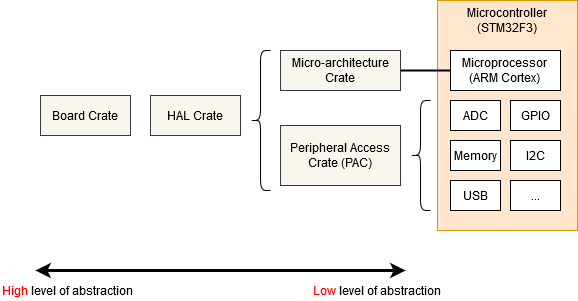
\includegraphics[width=\textwidth]{fig/crates.png}
  % Note: We do not have the SVG source file for the image above, so we have to put the PDF under version control.
  \caption{TODO: Create SVG}%
  \label{fig:embedded_crates}
  % Note: The `\label{}` can be on the line after the `\caption{}` if the `\caption{}` line ends with a comment.
\end{figure}

Since Rust appeared only very recently, the community already gained a lot of experience in embedded development.
Therefore, attempts were made to standardize and categorize embedded libraries.
There are several types of libraries, or crates, as they are called in Rust, see figure \ref{fig:embedded_crates}.
The most of the embedded libraries in Rust are strongly focused on the ARM Cortex-M architecture. Implementations for RISC-V microcontroller did exist, however, they are usually very minimalistic. See section~\ref{sec:libraries} for an overview of the necessary changes for RISC-V.

\subsection{Micro-architecture Crate (MAC)}
These crates handle any useful routines common to the processor core of a specific microcontroller, as well as any peripherals that are common to all microcontrollers that use that particular type of processor core. For example, the cortex-m crate gives features functions to enable and disable interrupts, which are the same for all Cortex-M based microcontrollers. It also gives you access to the 'SysTick' peripheral that is included in all Cortex-M based microcontrollers~\cite{RustEmbedded}. There also exists a very basic crate for RISC-V.

\subsection{Peripheral Access Crate (PAC)}
These crates are thin wrappers for the various memory-wrapper registers defined for a particular part-number of microcontroller. For example, stm32f30x for the ST-Micro STM32F30x series. Here, registers can be accessed directly, following each peripheral's operating instructions given in the microcontroller's Technical Reference Manual~\cite{RustEmbedded}.

\subsection{HAL Crate}
These crates offer a more user-friendly API for a particular processor, often by implementing some common traits defined in embedded \gls{hal}. It therefore makes use of the trait system, that could be compared to interfaces in Java. For example, this crate might offer a Serial struct, with a constructor that takes an appropriate set of GPIO pins and a baud rate, and offers some sort of \texttt{write_byte} function for sending data~\cite{RustEmbedded}. 

\subsection{Board Crate}
These crates go one step further than a \gls{hal} crate by preconfiguring various peripherals and GPIO pins to suit a specific developer kit or board, such as stm32f3-discovery for the STM32F3DISCOVERY board~\cite{RustEmbedded}.

\subsection{Runtime Crate}
These crates provide all code that is required to get to main. They usually feature either some low level Rust or even assembly code that initializes all registers, such as the stack pointer, setup interrupt vectors and finally call \texttt{main}. Furthermore, they provide macros to specify interrupt handlers. A RISC-V version of a runtime crate does exist, however only in a minimalistic version, without interrupt handler support.

\section{Interrupt Controller}
Since \gls{rtic} heavily relies on interrupts for tasks, it is also very dependent on a powerful interrupt controller hardware. Originally, \gls{rtic} was designed for \gls{nvic}

\section{NVIC}

\section{CLIC}